\documentclass[11pt]{article}
\usepackage[margin=1in, top=0.3in]{geometry}
\usepackage[all]{nowidow}
\usepackage[hyperfigures=true, hidelinks, pdfhighlight=/N]{hyperref}
\usepackage[separate-uncertainty=true, group-digits=false]{siunitx}
\usepackage{graphicx,amsmath,physics,tabto,float,amssymb,pgfplots,verbatim,tcolorbox}
\usepackage{listings,xcolor,subfig,caption,import,wrapfig}
\usepackage[version=4]{mhchem}
\usepackage[noabbrev]{cleveref}
\usepackage[T1]{fontenc}
\newcommand{\creflastconjunction}{, and\nobreakspace}
\numberwithin{equation}{section}
\numberwithin{figure}{section}
\numberwithin{table}{section}
\renewcommand{\subsectionautorefname}{section}
\renewcommand{\subsubsectionautorefname}{section}
\definecolor{stringcolor}{HTML}{C792EA}
\definecolor{codeblue}{HTML}{2162DB}
\definecolor{commentcolor}{HTML}{4A6E46}
\captionsetup{font=small, belowskip=0pt}
\lstdefinestyle{appendix}{
    basicstyle=\ttfamily\footnotesize,commentstyle=\color{commentcolor},keywordstyle=\color{codeblue},
    stringstyle=\color{stringcolor},showstringspaces=false,numbers=left,upquote=true,captionpos=t,
    abovecaptionskip=12pt,belowcaptionskip=12pt,language=Python,breaklines=true,frame=single}
\lstdefinestyle{inline}{
    basicstyle=\ttfamily\footnotesize,commentstyle=\color{commentcolor},keywordstyle=\color{codeblue},
    stringstyle=\color{stringcolor},showstringspaces=false,numbers=left,upquote=true,frame=tb,
    captionpos=b,language=Python}
\renewcommand{\lstlistingname}{Appendix}
\pgfplotsset{compat=1.17}

\begin{document}

\subsection{Scintillation detector theory}\label{sec:scintillator theory}
\autoref{sec:test}\autoref{sec:scintillators as triggers}
\subsubsection{Test}\label{sec:test}
\par The two scintillation detectors used in this experiment were constructed in 2018 and 2019 respectively \cite{2018 report}\cite{2019 report}. Their design is based on the detectors used in the HiSPARC project \cite{HISPARC}, which were designed to detect cosmic rays. 
\par The detectors built at UCT were made from an EJ200 scintillation plate, a photomultiplier tube (PMT), and a light guide. They each have a cross-sectional area of \SI{0.5}{\metre^2}. The 2018 detector is labelled with 1 gold star and the 2019 with 2.

% Insert a picture of one of the detectors.

\par As charged particles of a high enough energy enter the scintillation material, they excite electrons in the material which, as they de-excite, emit photons. These photons are always the same energy, so they hold no information about the energy of the charged particle, but the number of excited electrons, and thus the number of photons emitted, is proportional to the energy of the charged particle. 
\par The photons, if left unchecked, will be emitted isotropically, so they need to be guided towards the PMT in order to be detected. To do this, the scintillation material was covered in a reflective material and a light guide was fitted to one side of the scintillation material. This fed the photons onto the cathode plate of the PMT. 
\par Once the photons hit the cathode plate, they produce an electron by the photoelectric effect. This electron gets multiplied through an avalanche effect in the PMT before being output as a voltage pulse from the anode. Details on how scintillation detectors work and how they interact with PMT's can be found in \cite{Knoll} and details on the construction of the detectors can be found in \cite{2018 report} and \cite{2019 report}.
\newline
\par The primary use of the scintillation detectors is to trigger the TRD to begin recording data. This is so that we can be sure the TRD actually has something to detect. However, the scintillation detectors only tell us when a charged particle passes through the scintillation material of that specific detector. This tells us nothing about anything passing through the TRD, so we must turn to the theory of what we are detecting in order to proceed.
\par As described in [SECTION THAT TALKS ABOUT MUON SHOWERS], when muon showers occur, they usually result in straight lines of muons that travel parallel to each other. Using this knowledge, we can set up the scintillation detectors and the TRD such that any coincident pulses from the two detectors likely come from the same muon shower event, and thus we can be fairly certain a muon was passing through the TRD at the same time. We can then collect the data from the TRD corresponding to that event and analyse it as we please. The details of the set-up used are in \autoref{sec:scintillators as triggers}.

\subsection{Using the scintillation detectors as triggers for the TRD}\label{sec:scintillators as triggers}
\par The reasoning for choosing the set-up as we did is discussed further in [SECTION THAT TALKS ABOUT ANGULAR RESOLUTION], but \autoref{fig:scintillator setup} shows the set-up chosen. Ideally the two scintillators would be at the same height as the TRD chamber, but due to space constraints of the room housing the TRD chamber, they had to be placed [CAN'T REMEMBER THE DISTANCE RIGHT NOW] below the TRD chamber. Both scintillation detectors were at the same height.

\begin{figure}[h]
    \begin{center}
        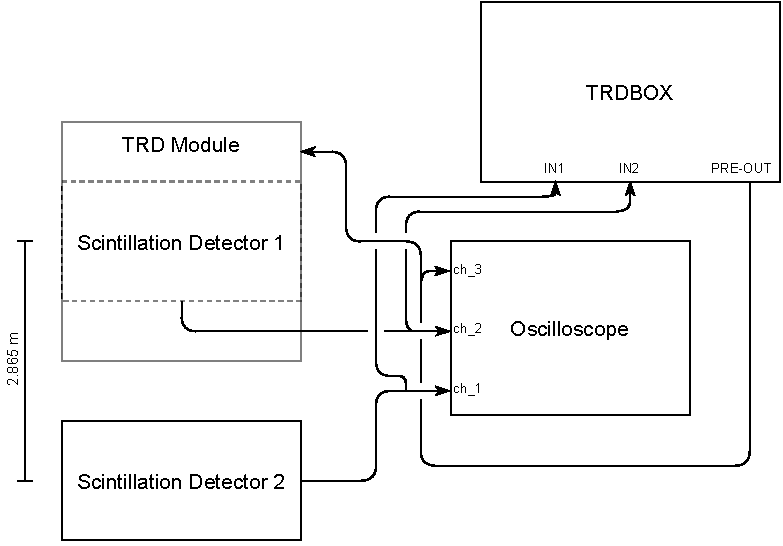
\includegraphics{Plots/setup.pdf}
        \caption{Simplified diagram of the set-up of the scintillation detectors with respect to the TRD chamber. Some details of the entire set-up have been left out, but this includes all the information relevant to the operation of the scintillation detectors as the triggers for the TRD chamber. Note that the TRD box output labelled "PRE-OUT" is the output that sends the trigger signal. Lengths are not to scale.}
        \label{fig:scintillator setup}
    \end{center}
\end{figure}

\par The two scintillation detectors sent their output signal to both the oscilloscope and the TRD box. Inside the TRD box, as described in [SECTION TALKING ABOUT DISCRIMINATORS AND TRIGGER SYSTEM], is a system which sends a trigger pulse when two signals from the scintillation detectors arrive within the specified time window. This trigger pulse goes to the oscilloscope as well as the TRD chamber. The oscilloscope was set to hold the data when it received a trigger, so that the details of the triggering event could be collected.  

\subsection{Scintillation detector operation}\label{sec:Scintillation detector operation}
\subsubsection{Oscilloscope set-up}\label{sec:Oscilloscope set-up}


\subsubsection{Collecting scintillation data}\label{sec:Collecting scintillation data}
\par In order to collect the data displayed on the oscilloscope, a modified version of the OpenWave-1KB \cite{Openwave} program was used. The version used can be found at \cite{Miles Git}, with a README outlining operation, as well as the quirks, but we will repeat the important parts here:
\par The oscilloscope can either be connected to the TRD computer directly using a USB cable, or over the network by ethernet. We strongly recommend using the USB connection as the interface written for ethernet had some very strange bugs that we weren't able to fix. The USB connection is not without its bugs but it works much better than ethernet. From this point on, instructions will be given assuming the USB connection is being used. This section will also reference the code in \cite{Miles Git}. The most important part of that repository is the \texttt{oscilloscopeRead} package. It has been written to be installed as a package on the TRD computer, just like \texttt{numpy} or \texttt{matplotlib}, and contains all the vital programs. The rest of the programs in the repository were written in order to actually use the \texttt{oscilloscopeRead} package to take data from the scintillation detectors. They can be used as is, with perhaps some modification of the filepath to save the data, or they could simply be used as an example for how the \texttt{oscilloscopeRead} package is best used. 
\newline
\par There are two methods of interfacing with the oscilloscope remotely. The first uses the \texttt{dso1kb} module. We found this method to be the most useful when we wanted to change specific settings on the oscilloscope, or just get to grips with the commands that the oscilloscope takes. This was best done within a python interpreter session (preferably within a venv that has \texttt{oscilloscopeRead} installed), and running the command \texttt{from oscilloscopeRead import dso1kb}. The name of the device in the system is then needed. This can be found by running \texttt{\$ dmesg} in the linux command line after plugging the oscilloscope into the TRD computer via USB, then looking for something that looks like this:
\begin{verbatim}
    [125714.945441] usb 3-8: Product: IDS-1074B
    [125714.945443] usb 3-8: Manufacturer: RS
    [125714.945444] usb 3-8: SerialNumber: 631D108G1
    [125714.956492] cdc_acm 3-8:2.0: ttyACM2: USB ACM device
\end{verbatim}

\texttt{IDS-1074B} is the oscilloscope, and \texttt{ttyAMC2} is the name needed. Now a \texttt{Dso} object can be created by running \texttt{dso = dso1kb.Dso(`/dev/ttyACM2')}. Note that the path to the device is needed, which should always be \texttt{/dev/}. After creating the object, commands can be sent to the oscilloscope using \texttt{dso.write(command)}. The commands that can be sent to the oscilloscope are all contained within the Programming Manual found in the Download section of \url{https://www.gwinstek.com/en-global/products/detail/GDS-1000B}. Some of the commands are used to change settings on the oscilloscope and as a result, do not return a value, however some of the commands, usually those that end in a ``?'', do return values. In order to access the returned value, \texttt{dso.read()} can be run in the python interpreter. This should return a byte string containing the returned value. Note that if the value is not read and another command is sent that also returns a value, it will be added to the buffer of returned values and running \texttt{dso.read()} will return the value from the first command. Reading again will then return the value from the second command. The command \texttt{dso.clearBuf()} can be used to clear the buffer entirely. 
\par A very important note about the commands being sent to the oscilloscope: When sending a command such as \texttt{:CHAN1:DISP ON}, which sets channel 1 to display, it is \textit{\textbf{ESSENTIAL}} that a line break character is added to the end of the command. In the python interpreter session, that would look like \texttt{dso.write(`:CHAN1:DISP ON\textbackslash n')}. Without this, the command will not be executed. 
\newline
\par The second method of interfacing with the oscilloscope, and the method we recommend when it comes to collecting data from it in conjunction with the data taken from the TRD chamber, is using the \texttt{scopeRead} module. This again requires the installation of the \texttt{oscilloscopeRead} package, but is best used in a python program. The \texttt{scopeRead} module contains a class called \texttt{Reader}. Creating a \texttt{Reader} object opens the connection to the oscilloscope, sets the oscilloscope to some settings that allow for good data, and then allows a few methods to be called. To create a \texttt{Reader} object, simply include the line \texttt{scope = scopeRead.Reader(`ttyACM2')} after importing the module. Note that here only the name of the device is needed, not the filepath. 
\par The methods that can be called are \texttt{scope.getData([1,2,3])} and \texttt{scope.takeScreenshot()}. The second of these simply takes a screenshot of the oscilloscope display and then saves it to the screenshots folder. The first method is the most important. It takes two arguments: A list of channel numbers to take data from, and an optional boolean value that tells the program whether to create a plot of the output and save it to the screenshots folder. The first argument needs to be a list of integers and can only contain the numbers 1 to 4. Numbers can be repeated, but this will simply return the same data. The default is the first three channels. The second argument is designed to be used as a debugging tool, not for data collection, and is by default set to False in order to not plot the data.

\begin{thebibliography}{9}
    \bibitem{2020 report} Arlow, H. Faul, S. Nathanson, N. Passmore, J. Pillay, K. Ramcharan, C. Roussos, G. Scannel, O. Thring, A. Wagener, J. Zimper, S. (2020). `Detecting and Tracking Cosmic Ray Muons using a Readout Chamber of the ALICE TRD'. UCT

    \bibitem{2019 report} Beetar, C. Blaauw, C. Catzel, R. Clayton, H. Davis, C. Diana, D. Geen, U. Grimbly, S. Johnson, D. Jackelman, T. McGregor, A. Moiloa, K. Oelgeschl\"ager, T. Perin, R. Rudner, B. (2019), `An Investigation Into the UCT-ALICE Transition Radiation Detector', UCT
    
    \bibitem{2018 report}  Barreiros, A. Barrella, J. Batik, T. Bohra, J. Camroodien, A. Govender, S. Lees, R. Rughubar, R. Skosana, V. Tladi, M. Wilkinson, J. Zeeman, W. (2018). `Detecting cosmic ray muons with an ALICE TRD Readout Chamber and commissioning a HiSPARC detector using electronic pulse processing'. UCT

    \bibitem{HISPARC} HiSPARC Project. Available at \url{https://www.hisparc.nl/en/} (2003)

    \bibitem{Knoll} Knoll, G. F., (2010). \textit{Radiation Detection and Measurement}. 4th ed. Wiley. New York.

    \bibitem{Openwave} GitHub - OpenWave-GW/OpenWave-1KB: A simple python program that can get image or raw data from digital storage oscilloscope (GDS-1000B) via the USB port. [online] Available at \url{https://github.com/OpenWave-GW/OpenWave-1KB}.

    \bibitem{Miles Git} GitHub - mkidson/ALICE\_LAB\_2021: The programs used to handle the scintillation detectors for the ALICE TRD lab 2021. [online] Available at \url{https://github.com/mkidson/ALICE_LAB_2021}.

    
\end{thebibliography}
\end{document}